\documentclass[fleqn,12pt]{article}

\usepackage{setspace,url,fullpage,latexsym,amsmath,amsthm,amssymb,pifont,graphicx,appendix,float,rotating,caption,subcaption,multirow,longtable,colortbl,natbib,graphics,graphicx,enumitem,pdflscape,epstopdf,verbatim,longtable}

\setcitestyle{aysep={},yysep={;}}
\bibliographystyle{apsr}


\usepackage{lipsum}
\usepackage{filecontents}
\usepackage[dvipsnames]{xcolor}
\usepackage{hyperref}
\usepackage[utf8]{inputenc}
\usepackage{cleveref}
\usepackage{pdflscape}
\usepackage{afterpage}
\usepackage{capt-of}
\usepackage{soul}
\hypersetup{
	backref =       true,
	pagebackref  =  true,
	colorlinks =    true,
	linkcolor =     blue,
	anchorcolor =   [rgb]{0.0,0.9,0.9},
	citecolor =     blue,
	filecolor =     [rgb]{0.0,0.1,0.7},
	urlcolor =      [rgb]{0.0,0.0,0.7},
}

% Packages for regression table
\usepackage{booktabs}
\usepackage{siunitx}
\newcolumntype{d}{S[
    input-open-uncertainty=,
    input-close-uncertainty=,
    parse-numbers = false,
    table-align-text-pre=false,
    table-align-text-post=false
 ]}

\doublespacing

\title{\singlespacing A Wiki-based Dataset of Military Operations with Novel Strategic Technologies (MONSTr)}
\author{J Andr\'{e}s Gannon{\thanks{Stanton Nuclear Security Fellow, Council on Foreign Relations, \texttt{jgannon@cfr.org}}} \\ Kerry Ch\'{a}vez{\thanks{Texas Tech University, Department of Political Science, \texttt{kerry.chavez@ttu.edu} \\
Previous versions of this paper were presented at APSA 2021 and 2022. For feedback on earlier drafts, the authors thank Jonathan Caverley, Rex Douglass, Erik Gartzke, Nadiya Kostyuk, Kendrick Kuo, Ashley Leeds, Erik Lin-Greenberg, Sara Plana, Thomas Scherer, Ryan Shandler, and Sanne Verschuren. Excellent research assistance was provided by Thomas Brailey, Zoe Coutlakis, Allison Lilley, Amanda Madany, Christie Marquez, David McCrum, Jordan Merkel, Matthew Miltimore, Dominick Nguyen, Peyton Olszowka, Cole Reynolds, Caitlen Rodriguez, Yiyi Sun, Qitao Wu, and Lisa Yen. This research was sponsored by Office of Naval Research Grant N00014-14-1-0071, the Department of Defense Minerva Research Initiative, the APSA Centennial Center, and the University of California -- San Diego Undergraduate Research Apprenticeship Program (URAP). Any opinions, findings, and conclusions or recommendations expressed in this publication are those of the author and do not necessarily reflect the view of the Office of Naval Research.}}}
\date{}

\usepackage{helvet}
\usepackage{titlesec}

\titleformat{\subsubsection}
{\normalfont\fontsize{12}{17}\bfseries\slshape}
{\thesubsection}
{1em}
{}

\begin{document}
	\maketitle
	\thispagestyle{empty}
	\setcounter{page}{0}
	
	\begin{abstract}
            \singlespacing \noindent Research on strategies and force structures in modern warfare is prolific, but siloed. While some examine boots on the ground, others focus on aerial bombing or unpiloted platforms. Consequently, most studies focus on the effects of one approach, seldom considering it in lieu of or conjunction with others. Furthermore, there is less knowledge on the origins and implementations of these strategic choices analyzed in isolation. The primary reason for these gaps lies with data limitations. This paper introduces a comprehensive dataset on the universe of United States military operations from 1989-2021 from a single source: Wikipedia. Using automated extraction techniques on its two structured knowledge databases$-$Wikidata and DBpedia$-$we uncover information about individual operations within nearly every post-1989 military intervention described in existing academic datasets. The data we introduce offers unprecedented coverage and granularity that enables analysis of myriad factors associated with when, where, and how the United States employs military force. We describe the data collection process, demonstrate its contents and validity, and discuss its potential applications to existing theories about force structure design and strategy in war.\\
		\vspace{.1in}
		\noindent
		\textbf{Keywords:} military intervention, use of force, dataset
	\end{abstract}
	
\newpage
\noindent

Despite being critical of the War on Terror, United States (US) President Obama amplified it upon assuming office and personally ensconced himself in the drone ``kill list" approval chain. Then-Director of National Intelligence Blair explained this pivot: ``It is the politically advantageous thing to do$-$low cost, no US casualties, gives the appearance of toughness” \citep{becker_secretkilllist_2012}. Critics argue that these benefits are outweighed by strategic costs such as backlash, radicalization, and increased terrorist recruitment \citep{kilcullen_opiniondeathoutrage_2009}. Obama's decision was not, however, whether or not to use drones. It was whether to use drones rather than insert or maintain boots on the ground in the ongoing wars in Iraq and Afghanistan that he campaigned on ending. It was whether to use drones rather than piloted flights outside of active war theaters.
	
Current research on how states use military force either focuses on the most aggregate level of the war or explains a particular tool in isolation. Consequently, variation in how states design and deploy force structures over a multi-year campaign remains unexplained. So does the relationship between complementary or substitutable types of force. As a result, academic understanding of how states fight is limited, being highly generalized on one side and siloed into individual domains or platforms on the other. There is a sprawling gap between these, where the actual warfighting occurs. Scholars interested in the prosecution of conflict contend with a dearth of data on the means of force across a comprehensive list of military operations. This paper debuts our attempt to overcome it.

We seek to remedy these shortcomings by providing a dataset that captures the means of force across a more expansive universe of US military events using a familiar, yet under-utilized data source: Wikipedia. Existing datasets focus on higher levels of aggregation, namely the broad military intervention, in part because collecting information at a more granular level is intensive and oft incomplete.\footnote{For instance, \citet[549]{allen_understandingimpactair_2017} remark that ``[i]deally, the unit of analysis for this project would be at the campaign level. Unfortunately, while most modern Western militaries operate in terms of campaigns, data for all countries over time was [sic] not available at the campaign level”.} Aware of the stigma attached to Wikipedia, we nonetheless note that what we gain is worth the tradeoffs. By scraping the Wikiverse for pages on post-1989 US military operations that occurred under the auspices of an intervention, our dataset identifies over 300 observations that existing datasets aggregate into broader wars. Using Wikidata and DBpedia, the structured bedrocks of Wikipedia, we also extract a host of fine-grained covariates concerning each military operation's dates, belligerents, location, and means used. Since these variables are less subject to human interpretation than those like conflict outcome or objective, concerns about data quality froma  source generally considered taboo are mitigated (though still addressed). We hope to convince that such a Wiki-based dataset on Military Operations with Novel Strategic Technologies (MONSTr) is not such a monster after all.

The paper proceeds with a section on our motivation, in which we trace the mismatch between our research interests and existing theory and data. Next, it outlines our approach in collecting, validating, and organizing the data gleaned from our Wikipedia extraction endeavor. Following this, we describe the dataset's distinctive features to convey the value added, suggesting how scholars might use them to extend or improve studies on how combatants fight. Specifically, we detail its increased granularity and depth, measures of the means of force for each operation, geographic precision, and thoroughness in identifying the roster of combatants on all sides. The penultimate section presents a data demonstration, predicting the means of military force with theoretically derived determinants drawn from existing scholarship. We conclude with a summary discussion, admission of limitations, and suggestions for future research using the MONSTr dataset.

\section*{Motivation}
A central question in international security concerns how strong states fight, and why. Sometimes they choose losing strategies against weak actors \citep{arreguin-toft_howweakwin_2001}. Military myopia arguments \citep{gentry_doomedfailamerica_2002, lyall_ragemachinesexplaining_2009}, capital-rich force structure narratives \citep{gartzke_democracypreparationwar_2001, caverley_mythmilitarymyopia_2009}, and uncertainty in pre-war estimates of costs and success \citep{sullivan_militaryinterventionpowerful_2009} explain many of these cases. Yet sometimes, despite bureaucratic inertia, economic factor abundance, and the fog of war, advanced militaries deploy ideal force structures against innovative weak enemies. Empirical tests of these theories are limited, however, by inadequate data required for validation. 

We identified three barriers to testing theoretical models of how states fight with existing data. First, we are interested in the planning and execution of military strategy \textit{during} armed conflict \citep{wallace_alliancesinstitutionaldesign_2008}. Most of the research and data has focused on its beginning$-$bargaining, causes, onsets$-$and end$-$duration, outcomes, aftermaths. Notwithstanding the profound knowledge they have yielded, these approaches black box the prosecution of war. This is surprising since we think its conduct has much to tell us about its causes and consequences. Some studies breach the black box of military force to analyze specific technological approaches within, but typically focus on the possession of platforms rather than their use, offering insight only on the latent potential for force \citep{gannon_planestrainsarmored_2021}.\footnote{Recent exceptions that focus on use include \citet{martinezmachain_aircampaignduration_2015}, \citet{post_flyingfailcostly_2019}, and \citet{gannon_oneifland_2022a}.} Furthermore, the majority bore a peephole onto a single platform or force structure rather than pop open the box. Some look at nuclear platforms \citep{gartzke_determinantsnuclearforce_2014}, naval power \citep{crisher_powerseanaval_2014}, aerial bombing \citep{pape_bombingwinair_1996}, air power more broadly \citep{horowitz_whendoesaerial_2001, martinezmachain_aircampaignduration_2015, allen_understandingimpactair_2017}, ballistic missiles \citep{reiter_ballisticmissilesinternational_2013}, cruise missiles \citep{early_climbingladderexplaining_2022}, or drones \citep{fuhrmann_droningexplainingproliferation_2017}.

This leads to the second barrier$-$siloed scholarship that inhibits the idea of substitutability \citep{morgan_modelforeignpolicy_2000}. At a high level, the substantial foreign policy literature reflects this standpoint by depicting a state's toolkit in broad categories$-$military, diplomatic, economic, cultural, etc. That same logic applies within each category. Leaders craft the use of military force not as isolated dichotomous decisions, but from a menu of substitutable (or complementary) options. Being domain- or platform-specific, existing datasets on the means of force are difficult to harmonize. Rather than peepholes into the blackbox of military force, our research questions on force structure and strategy require it to be open and well-lit. Once again, our inquiries on how and why states fight fall between existing theory and data, generalized on one side, specific but partitioned on the other.

Finally, holding the universe of military actions and the idea of substitutability in mind, a concern about the relationships across observations crops up. If we seek to explain why an operation featured solely unpiloted systems, it is relevant if it is part of a decapitation campaign in enemy territory. Or if a sizable contingent of troops is deployed for a manpower surge in Iraq, we naturally expect operations nested within the surge campaign to feature a higher frequency of ground troops. While scholars recognize this theoretically, existing datasets rarely identify the bureaucratic and strategic relationships of wars, campaigns, and operations. Testing explanations of force structure choices outside the strategic contexts in which they occur might lead to bias in estimating independent causal impacts.

\section*{Our Approach}
To surmount these barriers, we produced a dataset that features 1) measures of the means of military force across 2) a comprehensive and disaggregated list of US military operations that 3) captures dependence between observations using a consistent unit of analysis. Given the labor-intensive nature of manual data collection, we turned to the structured knowledge graphs of a familiar, underutilized source of information on political events: Wikipedia. There is virtually no scholar who promotes Wikipedia citations, but there is also virtually no scholar who does not queue up a Wiki page for initial information about a topic. While expert knowledge is required to measure contested or complex concepts like conflict outcome or purpose, it is less necessary to identify objective datapoints like the location, participants, and dates of an event. When collected carefully, we contend that the dimensionality and depth of such information easily extracted through automated processes is worth the taboo trade-off.

We disciplined our collection efforts definitionally, in space, and in time to curate a dataset on US military operations from 1989 to January 2021. The unit of analysis is the military operation. There is consensus among academics, practitioners, and military personnel that there are three general levels of conflict: strategic, operational, and tactical \citep{clausewitz_war_1976, millett_effectivenessmilitaryorganizations_1986, zabecki_german1918offensives_2006}.\footnote{These levels are generalized for conceptual clarity, but boundaries between them can be blurry in reality. In defining the levels of warfare, US military Joint Publication 3-0 acknowledges that ``there are no fixed limits or boundaries between these levels, but they help commanders visualize a logical arrangement of operations, allocate resources, and assign tasks to appropriate commands” 
 \citep[I-12]{chairmanofthejointchiefsofstaff_jointpublication30_2018}.} While scholars study all three, most research and datasets address the strategic level where national policy and theater planning dwells \citep{mcmaster_derelictiondutyjohnson_1998, millett_lessonswar_1988}. Meanwhile, most military studies focus on the tactical level where soldiers make decisions, execute tasks, and learn \citep{harkness_militarymaladaptationcounterinsurgency_2015, kollars_warhorizonsoldierled_2015}.

Since we are interested in phenomena between, our dataset dwells at the operational level that ``links the tactical employment of forces to national strategic objectives…using operational art to determine how, when, where, and for what purpose military forces will be employed" \citep{chairmanofthejointchiefsofstaff_jointpublication30_2018}. \citet{luttwak_operationallevelwar_1981} asserts that ``the operational level of war, as opposed to the tactical and strategic levels, is or ought to be of greatest concern to the analyst" (61). Several scholars agree that this level is more appropriate for studying military strategy and force structures \citep{allen_understandingimpactair_2017, tecottmetz_casecampaignanalysis_2021}. While it includes both operations and campaigns (series of related operations), MONSTr is organized according to the former since military doctrine identifies operations as the primary building block of this level. We follow the Department of Defense (DoD) dictionary which defines the operation as ``a sequence of tactical actions with a common purpose or unifying theme” \citep[GL-13]{chairmanofthejointchiefsofstaff_doddictionarymilitary_2021}.

Most existing datasets use the military intervention as the unit of analysis. To properly scope operations that fall within military interventions, we lean on the definitions in the exemplary Military Intervention by Powerful States (MIPS) and International Military Intervention (IMI) datasets. Like MIPS, we exclude threats, training exercises or mobilizations that demonstrate rather than apply force, ebbs and flows of personnel and materiel at permanent military bases, diplomatic cover and evacuation, and humanitarian operations \citep{sullivan_militaryinterventionpowerful_2009}. IMI clarifies that events must be purposeful and political \citep{pearson_internationalmilitaryintervention_1993, kisangani_internationalmilitaryintervention_2008}. Thus, we omit accidental and unintentional clashes. For instance, if troops deployed along the Iraq border have an unexpected encounter with Syrians, we view it as simply that—a military operation in Iraq that entailed a contingent clash with Syrians who meddled at the border. Being outside the politically determined mission scope, such a clash (or airspace violation) does not constitute a separate observation. We generated our original list of Wiki events to scrape from interventions identified in these reputable datasets. Table A2 in the Appendix summarizes our nearness to MIPS and IMI across definitional fine points of military intervention, and our departures from the broader approaches of RAND \citep{kavanagh_characteristicssuccessfulmilitary_2019} and Military Intervention Project (MIP) \citep{kushi_introducingmilitaryintervention_2022}. 

Combining the gold standard DoD definition of a military operation with the scoping conditions of a military intervention from MIPS and IMI, an observation in our dataset is:

    \begin{quote}\singlespacing
    \textit{A series of tactical actions (battles, engagements, strikes) conducted by combat forces in an operational theater to achieve strategic or campaign objectives in the context of a political issue or dispute through action against a foreign adversary. Routine military movements and operations without a defined target like military training exercises, the routine forward deployment of military troops, non-combatant evacuation operations, and disaster relief are excluded.}
    \end{quote}

With our focus on military operations, our dataset does not include drone strikes conducted by the Central Intelligence Agency (CIA), often in noncombat zones, even though they might be conceptualized as part of a military intervention. Falling outside the purview of the Pentagon, we contend that CIA operations abide by different constraints and covertness. In fact, extensive criticism has been levied at the CIA program for its lack of military control and transparency. 

Considering covertness, by nature of being collectible from the internet our cases are open source. We find this coverage appealing in that the events it includes have met some threshold of public awareness to make it onto Wikipedia. Since we expect that public attitudes amid the domestic politics of war are meaningful factors in how states fight, we accept this bias. There are interesting questions about the deployment of covert force, but we appreciate former Department of Intelligence Director Wilson's comment that ``90\% of intelligence comes from open sources. The other 10\%, the clandestine work, is just the more dramatic. The real intelligence hero is Sherlock Holmes, not James Bond" \citep{lands_publiclyavailableinformation_2019}. It's elementary$-$we leverage the data that are available and focus on research puzzles that interface with public attention and scrutiny.

Next, we spatially confined our sample to cases featuring the United States. Insofar as our impetus to collect these data is to examine how strong states fight, the US is a paragon. Its prolific intervention record also allows us to maximize observations in a pilot probe with one case. The US case is also deeply studied and data rich, better allowing us to test our theories and compare findings. Finally, we temporally confined our scope to start in 1989, when the US first used cruise missiles in conflict. With a special interest in the politics of emerging technologies, we aimed to collect a sample with temporal consistency in the military options, from ground troops to unmanned platforms, available to conflict decision-makers.

Of course, many of these scope limitations can and should be relaxed. Theoretical debates about how states fight would benefit from empirical information concerning pre-1989 interventions, non-US interventions, and a more expansive definition of military force (humanitarian aid, diplomatic evacuation, etc.). The dataset presented here is a proof of concept for the validity and value of using Wikipedia to identify and structure such information using comparatively feasible conditions. Future iterations of the project will expand in precisely these directions. In the following section, we describe the data collection process, with an emphasis on justifying our source, before demonstrating the data's yields and potential.

\section*{Dataset Inputs}
\subsection*{\textit{Collection - Scraping and Patching}}
For most readers, the Wiki interface is familiar. An executive summary sits under the page name, followed by a more detailed description of the entity, event, or concept. Most pages also contain an infobox containing a summary of attributes. For example, the ``cosmic latte" page informs that this is the average hue of the universe based on spectral analysis of over 200,000 galaxies. The sections describe the discovery and naming of the color.\footnote{Thank goodness ``primordial clam chowder" didn't win.} These data, like most other sources available to scholars, are unstructured and require manual review and entry.

Unlike most other natural language sources, Wikipedia rests upon two Resource Description Format (RDF) databases: Wikidata and DBpedia \citep{malyshev_gettingmostout_2018}. Wikidata contains an ontology for over 99 million items and their properties as ``triples." Each unique numeric identifier features a structured 1) subject, 2) predicate, and 3) object. For example, Germany (subject) has the capital (predicate) of Berlin (object). DBpedia maps information from each page's infobox also as structured content that can be semantically queried. Since both databases exist in a uniform, machine-readable format, we were able to scrape a comprehensive list of Wikipedia pages describing a US military operation from 1989 onward using SPARQL, an RDF query language. The resulting data contained nearly 500 entries and dozens of columns containing structured information from Wikidata and DBpedia infoboxes. After reasonable efforts to clean and process the queries as well as locate missing data from alternative sources, the neonate MONSTr had few holes.

\subsection*{\textit{Cleaning - Auditing and Validating}}
The primary contribution of our research method also constitutes its greatest burden: justifying Wikipedia itself. It carries a strong stigma in scholarly research that will be difficult to shake \citep{becker_researchfauxpas_2015}.\footnote{Please go read the entertaining opening of this short article, which we concede is better than ours.} We submit that for certain types of information it is a useful source. Our efforts to audit and validate the data took two forms: 1) an examination of scholarly research on Wikipedia's own data collection process and validation and 2) our own targeted and random audits of the Wikipedia pages that comprise MONSTr.

Although the use of Wikipedia in social science research remains relatively nascent, much has been done to evaluate its validity and reliability \citep{greenstein_wikipediabiased_2012}. In studies of over 10,000 randomly selected articles, scholars found Wikipedia’s accuracy on fact-based claims to be comparable to the Encyclopedia Britannica, the Dictionary of American History, and American National Biography Online using predictors such as page length, number of citations, external links, and edit history \citep{rector_comparisonwikipediaother_2008}.\footnote{Contrary to many course syllabi, Wikipedia vandalism is not as common as alleged: 81\% of uncited claims are flagged by bots using automated vandalism detection within 24 hours and fixed within three hours \citep{tramullas_researchwikipediavandalism_2016}.} Specific to political science, a study on Wikipedia’s coverage of 246 major-party gubernatorial candidates contained no errors in candidate biographies and 242 out of the 246 (98.4\%) reported election results within 0.2\% of the actual outcome \citep{brown_wikipediadatasource_2011}. Validation exercises on party ideology data from Wikipedia similarly deem that it bears correct, consistent information \citep{herrmann_partypositionswikipedia_2021}. Inconsistencies between (and within) Wikipedia and other sources largely pertain to frequently disputed figures (i.e., the precise size of armed forces in a battle) and more subjective interpretations (i.e., rationales and contested effects), datapoints that all sources struggle to pinpoint \citep{oswald_clickclickboom_2022}.

In addition to its accuracy, scholars have also evaluated Wikipedia's coverage. Wikipedia decides if an event should have its own page based on a criteria of ``notability."\footnote{Inclusion criteria differ by page type. All observations in MONSTr fall under ``events," for which inclusion criteria is detailed at \href{https://en.wikipedia.org/wiki/Wikipedia:Notability_(events)}{Wikipedia:Notability (events)}.} An event is considered sufficiently notable to have its own article if it ``has lasting major consequences or affects a major geographical scope, or receives significant non-routine coverage that persists over a period of time. Coverage should be in multiple reliable sources with national or global scope." Whether a page meets this criteria is decided by a combination of human editors and bots that evaluate the quality of new pages. Known biases in what meets these criteria have been uncovered, including a bias towards inclusion of recent events \citep{royal_whatwikipediawhat_2009} and those relevant to the English-speaking and Western world \citep{callahan_culturalbiaswikipedia_2011}. Comparisons can be drawn to media sources that have known biases in coverage of conflict \citep{dietrich_knownunknownsmedia_2020, croicu_reportingnonfatalconflict_2022}, which can impact event datasets that scholars use by biasing their sample, detail, and accuracy \citep{douglass_connectingconflictdata_2022}. Attempts to compare Wikipedia's coverage to news sources are complicated by their increased endogeneity, as news sources now use Wikipedia to decide what to cover \citep{ren_itnotencyclopedia_2023}. Nonetheless, Wikipedia's use of nonprofit, scholarly, and government sources as well as its ability to update pages based on new information means it is often more complete than media sources and also covers events that were only revealed or determined to be important well after they occurred \citep{gildersleve_newshistoryidentifying_2022}.

In addition to front-end and process audits, the authors manually checked variable values for a randomly selected sample of 6\% of all observations prior to identifying the operation-level ones. Validation sources stemmed from three sources. First, after consulting with personnel from all four of the major military branches to identify reputable government sources containing information on military operations. Second, in cases where none of the selected government or military sources contained information about an operation, we turned to reputable think tank and NGO reports or news outlets. To avoid circularity in validation, we were mindful to select news outlets that were not themselves cited in the Wikipedia article, although that was not possible in a few instances. We also filed two Freedom of Information Act (FOIA) requests to obtain After Action Reports (AAR), Battle Damage Assessments (BDA), and ship deck logs for known cases where little open source evidence existed. With the exception of uncertainty about the precise end date of two observations and whether one operation was against al-Qaeda or al-Qaeda and the Taliban, Wikipedia's coding for all other values could be independently verified. The manual audits also shed light on Wikipedia's coverage and inclusion criteria. Small and uneventful military operations were more likely to be listed as a subheader on an existing page or in a table with a brief summary, resulting in their exclusion from MONSTr. Contrary to findings about Wikipedia's Western and in-group bias, operations featuring high civilian casualties or misidentified targets usually appeared more detailed than those where the US accomplished its operational objective. A full description of the manual validation process is provided in the Appendix.

\subsection*{\textit{Clustering - Dependencies and Levels}}
Existing datasets on military intervention rarely record the relations between cases. This limitation can complicate the ability to analyze decision-making in the same dependent, dynamic context as political and military leaders. As an example, while MIPS, ICB, and MIDs have one observation for the two-decade War in Afghanistan, IMI considers the attacking and peacekeeping portions separately and RAND includes Operation Enduring Freedom (OEF), Operation Swift Freedom, International Security Assistance Force, Resolute Support and Freedom's Sentinel. In reality, Operation Swift Freedom was \textit{part of} OEF - Afghanistan, Freedom's Sentinel was a sub-campaign of Resolute Support, and of course all of these occurred under the umbrella of the Afghanistan War.

Since MONSTr delves into the operational level, we regarded a particular urgency to capture the higher levels in which each observation is situated. For each case, Wikipedia identifies a ``part of" variable that indicates the broader event to which the former is a subset. The level of ancestors (or higher levels of aggregation) for each operation varies. Some simply have one: Operation Uphold Democracy is part of the 1991 Haitian coup d'état. Others have more: the December 2018 airstrikes in Gandarshe are part of the American intervention in Somalia, which is a part of OEF – Horn of Africa, which is part of OEF. This Wikipedia feature enables us to identify and code the campaign and strategic levels in which each operation ought to be nested. To accomplish this, we constructed a dendrogram of the entire dataset, the trunk being any US military intervention in our time period and each branch being an increasingly intricate disaggregation from strategic to operational to tactical levels. We then independently and manually audited all 491 lines to cull operations, paring events at the tactical level, ensuring definitional accuracy, and validating ancestors. This resolved ambiguity for observations that were a part of multiple events, as one could be identified as the immediate parent (War in Afghanistan) and the other a higher level ancestor (War on Terror).

Notably, Wikipedia page names are not always an indication of the event level. They sometimes represent military designations and sometimes public labels. Technically, wars contain campaigns, which contain operations, which contain battles. In Wiki terminology, some entries entitled ``Operation” are not operations according to the DoD definition, some events bearing names like ``Battle of” are operations, and at times operations are nested within campaigns that are labeled as battles. For instance, Operation Euphrates Shield is a broader campaign containing four operations featuring alternative labels, like the East Aleppo Offensive (2017) described as a military operation to capture the Islamic State stronghold of Dayr Hafir and gain control of the city’s water source and airbase. As another example, the Battle of Panjwaii is a two-phase campaign to withstand Taliban forces in the district composed of two operations—Zahara and Medusa. Similarly, the RDF labels for ``instance of" abide by the same nomenclature inconsistencies and cannot be used to determine the case inclusion, which was instead done by the authors.\footnote{For example, Operation Vigilant Sentinel is an instance of ``conflict" while Operation Northern Watch is an instance of ``military operation." For a more thorough evaluation of the scope and relationships of conflict labels in Wikipedia, see (citation redacted).} During our operation identification exercise, we focused on the series of actions and levels of objectives rather than the Wiki names or sizes of events. For any discrepancies, we subjected cases to further scrutiny and debate until reaching consensus. The hierarchical relationships are a unique feature of our dataset that yields several advantages. It allows us to code, for example, how many days into OEF did the 2018 airstrikes occur. Furthermore, it facilitates hierarchical models accounting for structural dependencies among operations borne of the same strategic campaign and parent-intervention fixed effects.

\section*{Distinctive Outputs}
\subsection*{\textit{Granularity of Coverage}}
As already acknowledged, there are several datasets on military interventions at the strategic level. We do not supplant, but supplement them by identifying the more granular operations within them. For instance, most existing intervention datasets have an observation for the 2003 Iraq War. Ours identifies military operations and codes covariates associated with the individual operations within that war, as shown in Table \ref{tab:tbl:comparison-sample}. By disaggregating the unit of analysis, MONSTr provides information on 313 operations representing the 65 unique US interventions covered in all post-1989 datasets combined. This dimensionality is imperative for understanding how states fight. Reaffirming the connection between the study of strategy and the empirical operation we have sketched from other academic and military publications, US Army Field Manual 100-5 (1993) states that strategic objectives and military battles are harmonized by \textit{operational} art. Like going to war with the Army you have rather than the one you want, scholars examining force structures have done the best they can with the data that exist. Armed with Wikipedia, we can now go to war against unanswered research questions with the data we want.

\begin{center}
	[ Table \ref{tab:tbl:comparison-sample} about here ]
\end{center}

\subsection*{\textit{Depth of Datapoints}}
In addition to increasing the granularity of existing data by improving the precision of our unit of analysis, we were able to extract more granular variables characterizing operations. Shown in Table \ref{tbl:comparison-1}, MONSTr stacks up well against existing datasets on objective factors. It features start and end dates for each operation down to the day and a count of casualties (including civilians) for each side. The dataset also contains indicators for seven different types of force, an improvement over blunt domain codings collected at the intervention level or focuses on a single type when it comes to our research questions. Most operations include geocoded latitude and longitude coordinates, facilitating finer spatial analyses. It also identifies all state and nonstate actors active in the operation, both initiators and targets. Notably, MONSTr does not feature information on the aim and outcome of events. Treading lightly through data norms, we recognize that there is subjectivity afoot in discerning factors like military versus political objectives, \textit{ex ante} and \textit{ex post} objectives, and in interpreting outcomes. Although Wikipedia often includes these variables, we exclude them absent reliable evidence that it would be an improvement over the existing state of the art.

\begin{center}
	[ Table \ref{tbl:comparison-1} about here ]
\end{center}

\subsection*{\textit{Means of Force}}
\citet[335]{hart_strategyindirectapproach_1967} defines military strategy as ``the art of distributing and applying \textit{military means} to fulfill the ends of policy." Although strategy involves more than simple force structure design and deployment, these are nonetheless crucial components. The dearth and incomparability of the means of force in existing datasets are a chief reason we turned to Wikipedia since we could extract this variable for each operation. After several iterations of coding, auditing, and refining, we observed a co-occurrence of seven main categories of force: ground troops, paramilitary, close air support, air to air combat, aerial bombing, cruise missiles, and drones. Although some intervention datasets identify naval events during this time period, those events are identified in MONSTr by how the target was attacked, rather than the launch point (ie cruise missiles launched from a destroyer are coded as cruise missiles and an island landing for a raid is coded as ground troops). We explain this choice and our divergence from all cases coded as naval elsewhere in detail in the Appendix, allowing scholars to recode relevant cases in MONSTr as naval if desired.

Each force structure has its tradeoffs. Boots on the ground are more versatile, discriminating in context, and effective at winning hearts and minds in counterinsurgent settings (when done well). At the same time, they are more directly exposed to enemy attack, implying higher casualties, and by numbers and interaction density alone more prone to natural human error. Manned aerial platforms reduce risks and a degree of error, but exchange this for context-specific and time-sensitive intelligence and population-centric social capital \citep{lyall_ragemachinesexplaining_2009}. Unpiloted platforms (cruise missiles and drones) represent the lowest tactical risk to troops but the highest political risks of blowback \citep{johnston_impactusdrone_2016} and downsides to decapitation campaigns \citep{price_targetingtopterrorists_2012}. In addition to risks and effects, each of these means differently signals resolve \citep{zegart_cheapfightscredible_2018}. Overall, having measures of the means of force grants us great purchase in the study of military force structures.\footnote{The amount of missiles fired or troops deployed was of initial interest, but accurate data, especially concerning ordnance, proved challenging.} Descriptive statistics for the types of force in the dataset and other select covariates feature in the online appendix.

\subsection*{\textit{Nested Interdependencies}}
Researchers have long expressed concern over un-modeled interdependencies between conflict events. While frequently acknowledged in theories, the empirical mismatch due to limitations in available data problematize the important inferences scholars can make. Leveraging the structure of Wikipedia’s internal architecture, we identified and coded the nested relationships for each operation. Figure \ref{fig:fig-dendrogram-1} illustrates the high degree of interdependence among operations in our dataset. Moving to the right disaggregates each node into the operations that are part of it. Figure \ref{fig:fig-nested-1} homes in on the 1991 Gulf War to provide a more focused example. The Gulf War can be decomposed into three broad approaches: the no-fly zones, liberation of Kuwait, and air campaigns. Each features several operations in support of its objective. Looking at the distribution of the means of force along the right side of the figure, the importance of controlling for strategic campaigns becomes apparent. Intuitively, the aerial-focused ones feature higher frequencies of air power while the liberation campaign involves more ground troops, often in tandem with close air support. Although Wikipedia’s nested dependencies are not a perfect mapping relative to military or political dependencies, they will help scholars to better model this vital trait. 

\begin{center}
	[ Figures \ref{fig:fig-dendrogram-1} and \ref{fig:fig-nested-1} about here ]
\end{center}

\subsection*{\textit{Geographic Information}}
Nearly all operations in MONSTr are geocoded with GPS coordinates or a local municipality indicating where the event occurred.\footnote{In cases where the exact location was unknown, additional sources were consulted to identify the location with the most precisely reliable location. Those sources and methods are documented in the dataset.} For spatial analysts and geographic information system (GIS) users, this opens a wealth of inquiries. For instance, it allows for the coding of terrain, which might influence the force structure deployed \citep{gleditsch_richardsoninformationage_2012, shaver_terrainruggednessland_2019}. It also allows analysis of urbanicity, proximity to strategic assets, adaptation amid shifting combat fronts, power projection, contagion, and more (limited only by GIS layers and imagination). In Figure \ref{fig:fig-map-1}, we plot the locations of the US operations in the dataset and identify one potential application -- the association between urban/non-urban targets and the type of military force used. Although merely descriptive, the types of force used in operations in Syria, Iraq, and Afghanistan raise interesting questions. Non-urban operations in Iraq appear to primarily involve ground troops except in the mountainous north, where aerial bombing dominates. The majority of US operations in Afghanistan occur in non-urban areas, with those crossing the Pakistan border constituting aerial operations typically associated with US drone strikes during the Obama administration. This descriptive evidence suggests ways in which these data could be used to test theories about the relationship between geography, target type, and the means of applications of military force.

\begin{center}
	[ Figure \ref{fig:fig-map-1} about here ]    
\end{center}

As a GIS-capable team, we are enthusiastic about these prospects. Still, as an intellectually honest team, we caution interpretations about the geography of US military operations from these data. First, Wikipedia does not distinguish between geometry type, which matters for events that occurred in multiple districts or towns. In these cases, we deferred to the coordinates provided by the DBpedia infoboxes to ensure a consistent protocol and to enable future researchers to compare this to other sources. In addition, we addressed non-random missingness using Google Earth data which also raises questions about the consequences of geographic coding using multiple gazetteers \citep{douglass_measuringlandscapecivil_2018}.

\subsection*{\textit{Actors Involved}}
The identity, traits, and connections of actors in conflict have a dramatic impact on how they fight. Scholars have long recognized and researched this \citep{huth_majorpowerintervention_1998}. Powerful states, more likely to have economic assets to protect and military ones to project power, intervene more frequently \citep{sullivan_militaryinterventionpowerful_2009}. Democracies might deploy force for different reasons, in different ways, and for different durations than autocracies \citep{caverley_democraticmilitarismvoting_2014, talmadge_differentthreatsdifferent_2016}. Some states are primarily compelled by security, some economy, some to contain spillover of violence or refugees, some drawn in by allies or against rivals, and some by humanitarian impulses.\footnote{The many good works exploring each determinant are too many to list here.} Considering intervenors alone, multilateral campaigns—distributing costs and risks across partners yet involving larger coordination challenges—require different calculus than unilateral ones. For example, in Serbia 1996 US generals realized that to keep the 19 North Atlantic Treaty Organization (NATO) allies on board, their preference of a saturated, decisive air campaign was off the table \citep{cooper_politicsairstrikes_2001}. Speaking only of targets, states might behave differently against nonstate combatants relative to fellow states. And in the same way that multilateral state coalitions change the fighting calculus, nonstate actors form complex and shifting coalitions too. The Syria Civil War, with its makeshift operations rooms and mercurial alliances, illustrates this well \citep{cranmer_coalitionqualitymultinational_2018}. In short, the consequences of intervention hinge on collective actor traits on both sides and interactions across \citep{carment_threecompanyevaluating_1998, caverley_mythmilitarymyopia_2009}.

While we know these factors matter, much analysis oversimplifies by looking at the primary intervenor and target. This masks important variation in participants, especially those occurring over years or even decades. The roster comprising the coalition throughout the Afghanistan War, for instance, oscillated over its life. Even if it remained constant, not all members participated in each operation, to the same degree, or for the same reason \citep{gannon_keepingyourfriends_2021}. Nor did the targets remain constant over the course of the conflict. At times, the US unilaterally deployed special forces against anti-coalition insurgents (Operation Red Wings). At other times, it pitched in beside Dutch pilots to provide close air support for Aussies and their Afghan mentees ambushed by the Taliban (First Battle of Kakarak). Unsurprisingly, the force structures selected for these events were quite different. Who fights, whom they are fighting alongside, and whom they are fighting against are important for explaining comportment in conflict \citep{cappellazielinski_understandingbattlefieldcoalitions_2022}.

Our data capture this variation in actor interaction as showcased in Figure \ref{fig:fig-actors-1}. These three network plots of the US and its partners (side A) feature state allies in green and nonstate actors fighting alongside the US in orange. The edges are weighted by the number of operations shared between dyads. Maintaining focus on the Afghanistan War, the top right panel portrays the many actors participating throughout the 20-year war. Intuitively, the US most densely interacted with the state of Afghanistan itself after ousting the Taliban. While key Western partners situate strongly in the network, direct US involvement with the United Kingdom (UK) was most prominent. Other interesting traits emerge in comparison to the 1991 Gulf War (top left) and the 2015 Syria Civil War (bottom left). First, the composition of US partners changed dramatically across these conflicts. All allies in the Gulf War were states. In Afghanistan, state partners remain the norm but plenty of nonstate actors joined the fray. In the Syria War, nonstate partners outnumber states two-to-one. Edges shared with the UK are thick throughout, but in Syria US cooperation with a nonstate actor eclipses it by a small margin. Interaction density between actors varies across conflicts as well, being straightforward and balanced in the Gulf, layered and feathery in Afghanistan, and sprawling and asymmetric in Syria. Even with only allies in only three strategic level interventions, we see intriguing patterns that spark questions. MONSTr affords the ability to analyze them in significantly more detail.

\begin{center}
	[ Figure \ref{fig:fig-actors-1} about here ]    
\end{center}

\section*{Demonstration}
As a proof of concept demonstrating the validity and value of these data, this section presents the results of statistical models based on existing theories about why states deploy particular military means. The goal of these models is to see how the new, more disaggregated data from a novel source compares to existing findings. While the more fine-grained unit of analysis makes an exact replication impossible, the results of these models should nonetheless provide evidence that is either consistent or inconsistent with existing research. Existing research analyzes the determinants of ground forces, air power, and a rare few examine the conditions of their combination. We emulate this to compare general patterns and findings. 

\subsection*{\textit{Specification}}
The unit of analysis is the US military operation. For the dependent variables, we take advantage of the disaggregated types of force available in our dataset. Thus, each model in Table \ref{tbl-results} features coefficients for a separate binary dependent variable indicating the use of a key means of force: \textsc{Ground}, \textsc{Air and Ground} in conjunction, \textsc{Air}, and subsets of air power to explore the use of \textsc{Piloted} and \textsc{Unpiloted} platforms.\footnote{Since 1) the dependent variables span the same range and 2) models stem from the same sample and feature the same explanators and specifications, we are on safe statistical ground to compare across models.} The dependent variables are binary and the data are nested, calling for a logit estimator in hierarchical models that account for the strategic dependencies of operations within each broader war.

We also build upon previously theorized explanators for state force structures. Past studies have examined factors such as target type, geography, and timing. First, we include an indicator for whether side B features a \textsc{Nonstate Target}, which tend to use different strategies to deflect the brute force of stronger state actors \citep{arreguin-toft_howweakwin_2001}. Second, we consider two geographic features that likely affect the feasibility of different force structures. \textsc{Mountainous} terrain is more difficult for foot soldiers to traverse, especially if combatants are advantageously embedded throughout. \textsc{Urban} settings are complex operating environments, dense with structures, sensitive infrastructure, and civilians, so might be less amenable to higher-tech means of force. Finally, strategies and force structure design might change over the life of a conflict. We include a \textsc{Duration} variable and a measure capturing how many \textsc{Days into the Parent} conflict the operation occurred, both logged to normalize their distributions. All models include president fixed effects to control for leader idiosyncrasy and cubic polynomials of the number of years since the dataset's start to control for nonlinear time dependence \citep{carter_backfuturemodeling_2010}.

\subsection*{\textit{Results}}
Model results are reported in Table \ref{tbl-results}. Concerning the target of US operations, it appears that those with nonstate combatants are much less likely to feature combined ground and air tactics or air power pooled. When it comes to geography, operations taking place in mountainous terrain are associated with more aerial bombing, bringing to mind the infamous 72-hour bombing campaign of the Tora Bora mountain caves targeting Osama bin Laden in late 2001. No clear association exists with urban targets, which runs counter to theories that drones' more precise and discriminating nature makes them well-suited to operations in complex environments dense with civilians. Instead, the US may avoid drone strikes in urban areas because of the domestic backlash to civilian deaths.

Intriguingly, longer operations are associated with an increased frequency of piloted air power, yet air operations do not seem to feature earlier in a conflict. These temporal variations warrant further consideration and theorizing. \citet{martinezmachain_aircampaignduration_2015} demonstrates that ground troops affect the duration of aerial campaigns divergently depending on how discriminate the latter's approach. While we don't observe that the days into the parent intervention affect force structure choices, suggesting that this hinges more on conflict dynamics than mere time, we do note that longer interventions tend to feature more ground, combined arms, and manned air power. Overall, the results mostly affirm conventional wisdom, but also point to new puzzles that the dataset will enable scholars to examine.

\begin{center}
	[ Table \ref{tbl-results} about here ]
\end{center}

\section*{Conclusion and Future Directions}
With the advent of automated extraction, and the audacity to apply it to a well-known yet long-avoided source, we were able to collect a first cut of data in a relatively easy and well identified sample as a proof of concept. The Wiki-based MONSTr dataset features objective correlates of the operations within nearly all US military interventions from 1989 to January 2021 in a nested structure reflecting observation interdependencies. Its unit of analysis is more granular, its depth more detailed, and its structure more realistic than existing sources. It also features the means of force used in each operation, opening avenues to explore fresh puzzles about the prosecution of conflict. We have scantly demonstrated the potential applications of these data, showing preliminary patterns of force using actor and event traits. Many findings accord with existing theory -- like the use of aerial bombing in mountainous environments -- while others provoke new ideas -- like an aversion to piloted bombing against nonstate targets and fewer drone strikes against urban targets.

We observe several avenues for future research, both theoretical and empirical. Theoretically, we wonder about the determinants of force structures, both retesting conventional wisdom and expanding it. In particular, we expect that domestic public factors constrain and compel the force structures of strong, democratic states. We also promote explorations of actor dynamics on both sides and across. As conflicts increasingly feature nonstate actors as partners and targets, future research can unpack how states fight alongside or against them given the asymmetry in strength and unconventional strategies. We also see potential to explore how operations change across the life of a parent conflict. Our demonstrative models suggest that the means of force shift the longer the intervention yet perhaps not depending on depth into the parent campaign. Conversely, scholars can examine the impact of force structures on domestic political moods, strategic leader behavior, partner configurations, duration, and more. We see value in analyzing the combinations of military means in tailored force structure packages. For instance, ground forces and close air support no doubt co-occur and unmanned air power likely flies alone more often than not. Empirically, despite the considerable expansion in coverage and granularity, our data are bounded in a brief time period for one nation. Data stretching further back and abroad are there, awaiting extraction. Given the machine-readable format, it is exceptionally easier to approach an endeavor of this scope than with manual efforts (once you learn SPARQL and Wiki's anatomy). 

There remain many research questions on how states fight. Scholars have done impressive work with limited data on the means of force, yet their siloed, specific nature and high levels of aggregation inhibit inquiry into the full, operational spectrum of military power. Especially since means of force are substitutable and combinable, understanding their interaction is critical to advance knowledge. On top of that, the practical assumption of independence across observations in existing datasets separates events that are strategically linked. Producing a dataset that overcomes these challenges and continues to offer the same depth and precision (in fact, more) seems Herculean. We are well aware and in great admiration of the painstaking, long-term efforts to stitch together data on military interventions from dozens of sources. Although we acknowledge Wikipedia's drawbacks, we maintain that, with transparency about these traits, we can learn a great deal about the conduct of war that we would otherwise not know. We have no expectation or hope that a Wiki-based dataset will replace or compete with others. We do, however, expect and hope that it will expand in coverage and use. Combined with more rigorous qualitative and quantitative approaches, we believe our data make a meaningful contribution to the social scientific and practitioner communities aiming to accumulate knowledge. We hope MONSTr grows. Many will choose not to use it but we hope in the end some will profess, ``I love you too much to condemn you” \citep{coppola_dracula_1992}.

\newpage

\thispagestyle{empty}
    \begin{landscape}
    \begin{table}

\caption{\label{tab:tbl:comparison-sample}Sample of Iraq War (2003) operations}
\centering
\resizebox{\linewidth}{!}{
\begin{tabular}[t]{l|r|r|r|r|r|r|l|l|r|r|r|r|r}
\hline
\multicolumn{1}{c|}{} & \multicolumn{4}{c|}{Means} & \multicolumn{2}{c|}{Location} & \multicolumn{4}{c|}{Time} & \multicolumn{3}{c}{Casualties} \\
\cline{2-5} \cline{6-7} \cline{8-11} \cline{12-14}
\textbf{Operation} & \textbf{Aerial bombing} & \textbf{CAS} & \textbf{Ground troops} & \textbf{Paramilitary} & \textbf{Lat} & \textbf{Lon} & \textbf{Start} & \textbf{End} & \textbf{Duration} & \textbf{Days into war} & \textbf{Side A} & \textbf{Side B} & \textbf{Civilian}\\
\hline
Operation Al Majid & 0 & 0 & 0 & 1 & 34.37222 & 41.98750 & 2006-09-01 & 2007-02-01 & 153 & 1261 & NA & NA & NA\\
\hline
Siege of Sadr City & 1 & 1 & 1 & 1 & 33.38993 & 44.46065 & 2004-04-04 & 2008-05-11 & 1498 & 381 & 325 & 3050 & NA\\
\hline
Operation Ardennes & 0 & 0 & 1 & 0 & 30.96083 & 46.10611 & 2007-06-17 & 2007-06-17 & 0 & 1550 & 0 & 0 & 0\\
\hline
Battle of Debecka Pass & 1 & 0 & 0 & 1 & 35.88426 & 43.78376 & 2003-04-06 & 2003-04-07 & 1 & 17 & 18 & NA & NA\\
\hline
Operation Iron Saber & 0 & 0 & 1 & 0 & 32.01066 & 44.32653 & 2004-04-01 & 2004-06-22 & 82 & 378 & 0 & 0 & 0\\
\hline
Operation Phantom Thunder & 1 & 1 & 1 & 0 & 33.22319 & 43.67929 & 2007-06-16 & 2007-08-14 & 59 & 1549 & 380 & 1196 & NA\\
\hline
Battle of Al Faw (2003) & 1 & 1 & 1 & 1 & 29.98117 & 48.46757 & 2003-03-20 & 2003-03-24 & 4 & 0 & 19 & 150 & NA\\
\hline
Operation Iron Triangle & 0 & 0 & 1 & 0 & 34.16600 & 43.90552 & 2006-05-09 & 2006-05-09 & 0 & 1146 & 0 & 4 & NA\\
\hline
\end{tabular}}
\end{table}
    
    \end{landscape}
\pagestyle{plain}
\setstretch{2.0}

\clearpage
\begin{landscape}
\thispagestyle{empty}
    	\begin{table}[ht]
	\begin{center}
		\caption{Comparison of Variable Granularity} 
		\label{tbl:comparison-1}
		\footnotesize
		\begin{tabular}{lcccccccccc}
			\hline \hline
			\noalign{\vskip 0.15cm}
			\textbf{Dataset} $\rightarrow$ & \textit{MONSTR} & \textit{MIPS} & \textit{IMI} & \textit{ICB} & \textit{MIDs} & \textit{MIP} & \textit{UCDP/} & \textit{RAND} & \textit{Allen} & \textit{Horowitz}\\
			\textbf{Variable} $\downarrow$ & & & & & & & \textit{PRIO} & & & \textit{\& Reiter} \\
			\noalign{\vskip 0.15cm}
			\hline
			\noalign{\vskip 0.15cm}
			\textit{Scope} & 1989-2021 & 1945-2001 & 1946-2005 & 1918-2015 & 1816-2010 & 1776-2019 & 1946-2018 & 1900-2015 & 1914-2003 & 1917-1999 \\
			\noalign{\vskip 0.15cm}
			\hline
			\noalign{\vskip 0.15cm}
			\textit{N (US, all dates)} & 336 & 35 & 109 & 71 & 325 & 392 & 18 & 145 & 49 & 17 \\
			\noalign{\vskip 0.15cm}
			\hline
			\noalign{\vskip 0.15cm}
			\textit{N (US, post-1989)} & 336 & 16 & 38 & 20 & 72 & 115 & 17 & 64 & 4 & 5 \\
			\noalign{\vskip 0.15cm}
			\hline
			\noalign{\vskip 0.15cm}
			\textit{Date} & day & day & day & day & day & day & day & year & year & year \\
			\noalign{\vskip 0.15cm}
			\hline
			\noalign{\vskip 0.15cm}
			\textit{Casualties} & count & count & count & ordinal & ordinal & count & - & - & - & - \\
			\noalign{\vskip 0.15cm}
			\hline
			\noalign{\vskip 0.15cm}
			\textit{Military Means} & all & ordinal & domain & - & - & domain & - & - & air, land & air \\
			\noalign{\vskip 0.15cm}
			\hline
			\noalign{\vskip 0.15cm}
			\textit{Geography} & geocoded & state & state & subcontinent & - & state & territory & state & - & - \\
			\noalign{\vskip 0.15cm}
			\hline
			\noalign{\vskip 0.15cm}
			\textit{Intervenors} & all & primary & primary & all & primary & primary & primary & primary & primary & all \\
			\noalign{\vskip 0.15cm}
			\hline
			\noalign{\vskip 0.15cm}
			\textit{Targets} & all & all & primary & primary & primary & all & primary & primary & primary & all \\
			\noalign{\vskip 0.15cm}
			\hline
			\noalign{\vskip 0.15cm}
			\textit{Target Type} & - & $\checkmark$ & - & - & - & - & $\checkmark$ & - & $\checkmark$ & - \\
			\noalign{\vskip 0.15cm}
			\hline
			\noalign{\vskip 0.15cm}
			\textit{Objective} & - & $\checkmark$ & $\checkmark$ & $\checkmark$ & - & $\checkmark$ & - & - & $\checkmark$ & $\checkmark$ \\
			\noalign{\vskip 0.15cm}
			\hline
			\noalign{\vskip 0.15cm}
			\textit{Outcome} & - & $\checkmark$ & $\checkmark$ & $\checkmark$ & $\checkmark$ & $\checkmark$ & - & - & - & $\checkmark$ \\
			\noalign{\vskip 0.15cm}
			\hline \hline
		\end{tabular}
	\end{center}
\end{table}
\end{landscape}
\setstretch{2.0}

\setstretch{1.2}
\clearpage
\thispagestyle{empty}
    \begin{table}

\caption{\label{tab:tbl-results}Exploratory Models of Determinants of Means of Military Force}
\centering
\begin{tabular}[t]{lccccc}
\toprule
  & Ground & Ground and Air & Air (all) & Air (Piloted) & Air (Unpiloted)\\
\midrule
Non-state target & \num{0.542} & \num{-1.251}** & \num{-1.787}** & \num{-1.501}** & \num{-0.336}\\
 & (\num{0.477}) & (\num{0.037}) & (\num{0.017}) & (\num{0.016}) & (\num{0.694})\\
Mountainous target & \num{-0.591} & \num{0.354} & \num{0.788}* & \num{0.509} & \num{0.225}\\
 & (\num{0.207}) & (\num{0.301}) & (\num{0.064}) & (\num{0.183}) & (\num{0.737})\\
Urban target & \num{0.339} & \num{0.300} & \num{0.156} & \num{0.314} & \num{-0.620}\\
 & (\num{0.412}) & (\num{0.373}) & (\num{0.675}) & (\num{0.356}) & (\num{0.289})\\
Duration (log) & \num{0.305}*** & \num{0.238}*** & \num{0.001} & \num{0.126}* & \num{0.015}\\
 & (\num{0.001}) & (\num{0.002}) & (\num{0.992}) & (\num{0.090}) & (\num{0.895})\\
Day into Parent (log) & \num{0.164} & \num{0.137} & \num{-0.037} & \num{0.016} & \num{-0.087}\\
 & (\num{0.267}) & (\num{0.289}) & (\num{0.784}) & (\num{0.892}) & (\num{0.632})\\
\midrule
Num.Obs. & \num{260} & \num{260} & \num{260} & \num{260} & \num{260}\\
R2 Marg. & \num{0.511} & \num{0.430} & \num{0.459} & \num{0.401} & \num{0.324}\\
R2 Cond. & \num{0.565} &  & \num{0.491} & \num{0.435} & \num{0.578}\\
AIC & \num{274.8} & \num{328.7} & \num{300.2} & \num{340.1} & \num{196.5}\\
BIC & \num{328.2} & \num{382.1} & \num{353.6} & \num{393.5} & \num{249.9}\\
ICC & \num{0.1} &  & \num{0.1} & \num{0.1} & \num{0.4}\\
RMSE & \num{0.38} & \num{0.44} & \num{0.41} & \num{0.44} & \num{0.28}\\
\bottomrule
\multicolumn{6}{l}{\rule{0pt}{1em}* p $<$ 0.1, ** p $<$ 0.05, *** p $<$ 0.01}\\
\multicolumn{6}{l}{\rule{0pt}{1em}All models include president fixed effects and cubic spline polynomials.}\\
\end{tabular}
\end{table}

\pagestyle{plain}
\setstretch{2.0}

\clearpage
\setstretch{1.0}
\newpage
\begin{figure}[h]
	\begin{center}
		\caption{Nested Dependencies of US Military Operations}
		{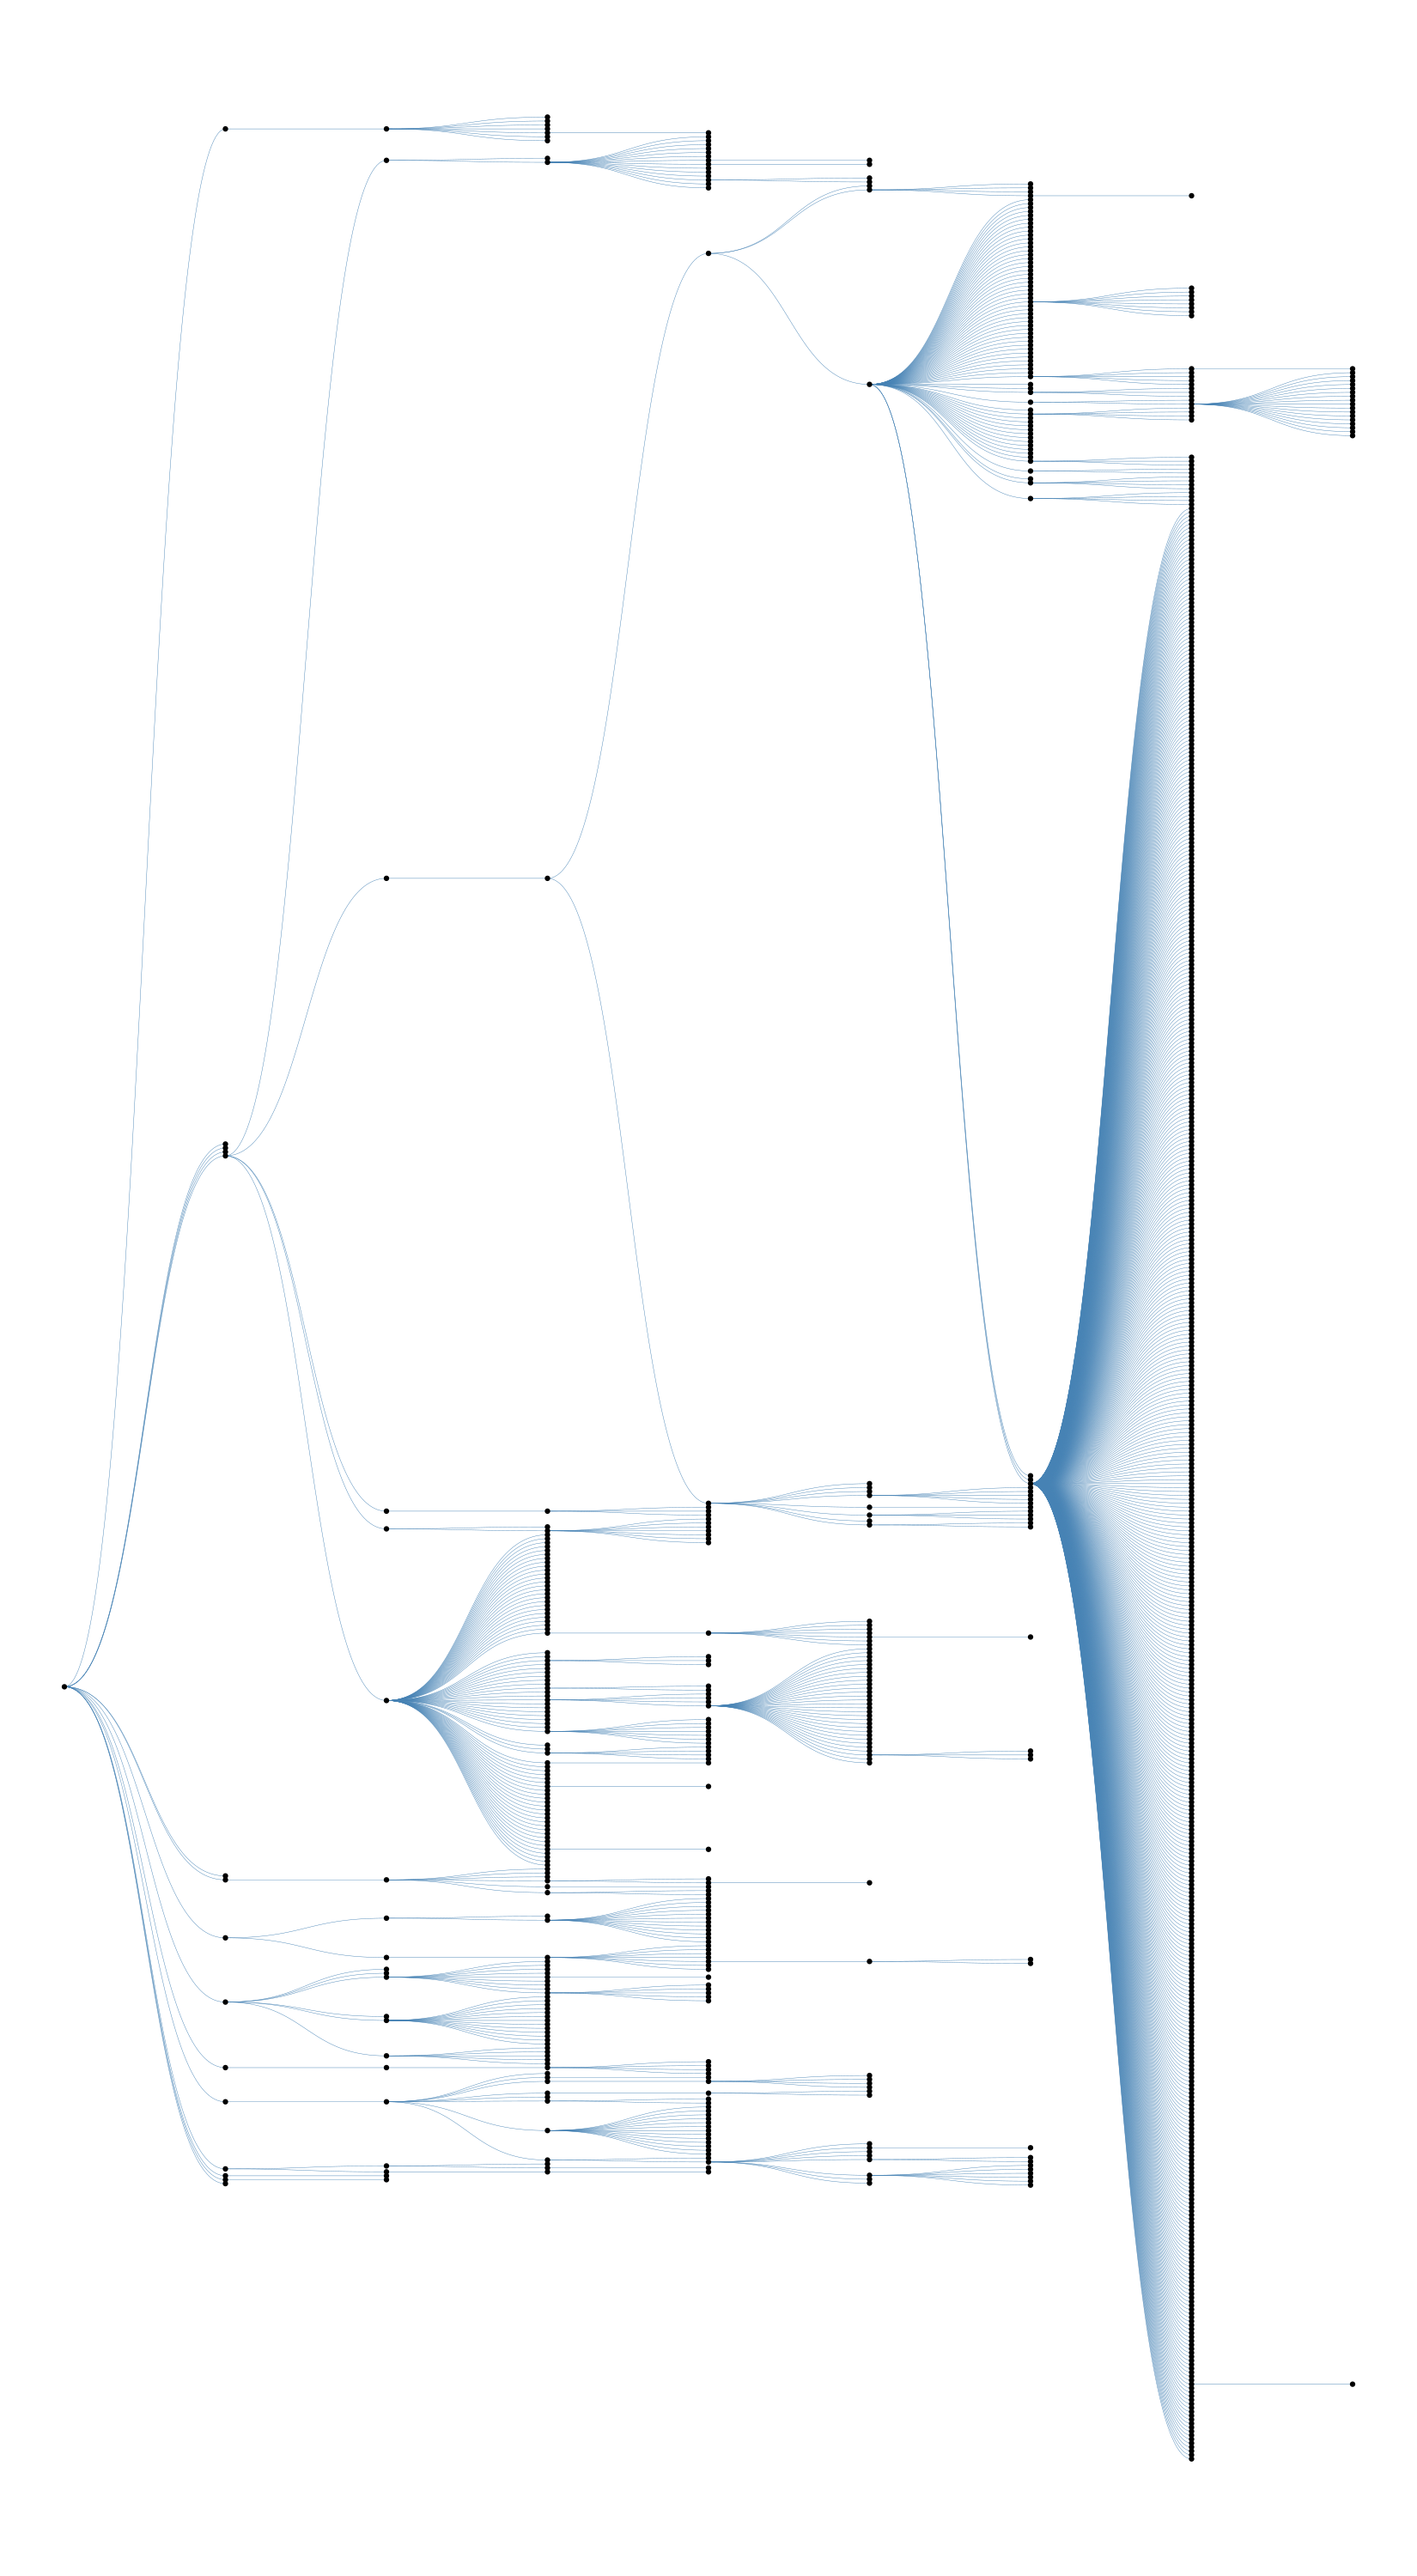
\includegraphics[height = \textheight]{fig-dendrogram-1.png}}
		\label{fig:fig-dendrogram-1}
		\vspace{0.1 in}
	\end{center}
\end{figure}
\setstretch{2.0}

\clearpage
\setstretch{1.0}
\newpage
\begin{figure}[h]
	\begin{center}
		\caption{Nested Structure of the Gulf War (1991)}
		{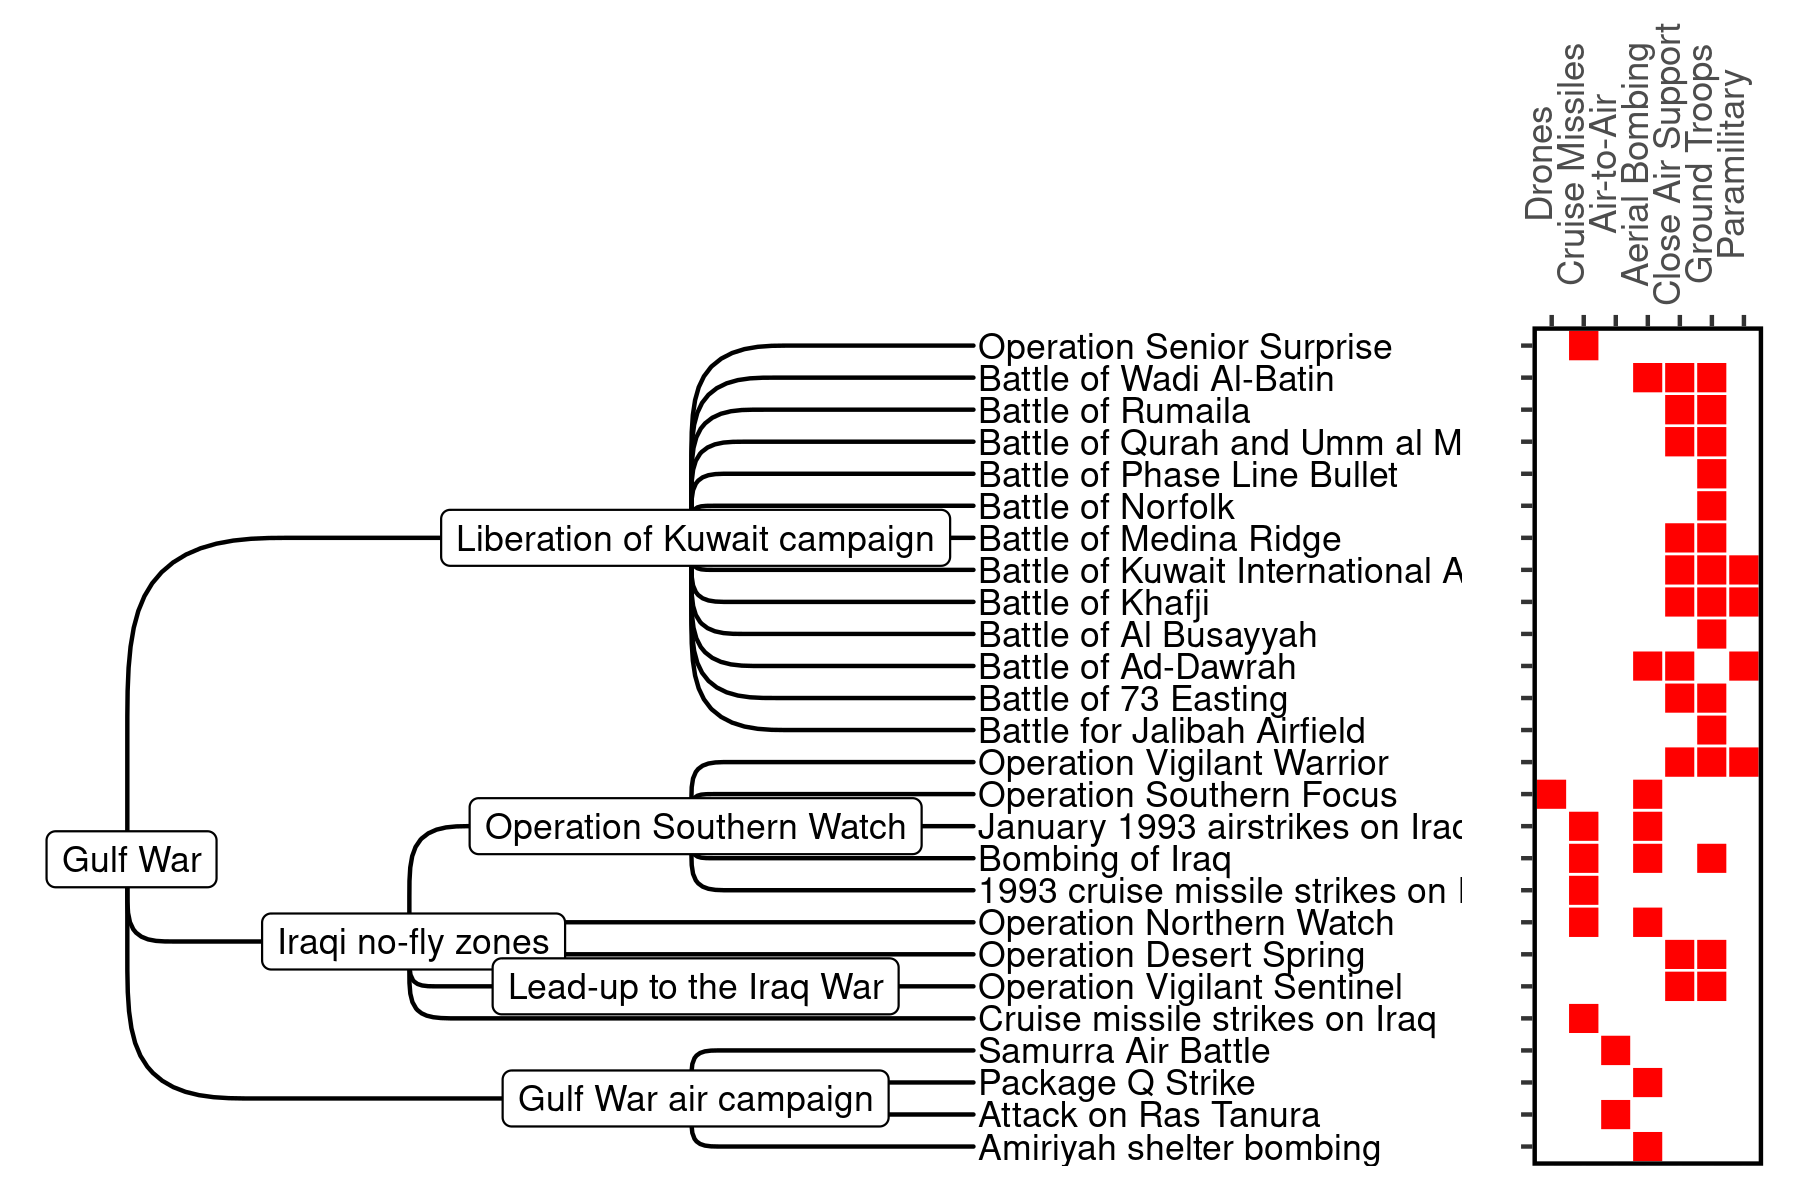
\includegraphics[width = \textwidth]{fig-nested-1.png}}
		\label{fig:fig-nested-1}
		\vspace{0.1 in}
	\end{center}
\end{figure}
\setstretch{2.0}

\clearpage
\setstretch{1.0}
\newpage
\begin{figure}[h]
	\begin{center}
		\caption{Locations of US Military Operations (1989-2021)}
		{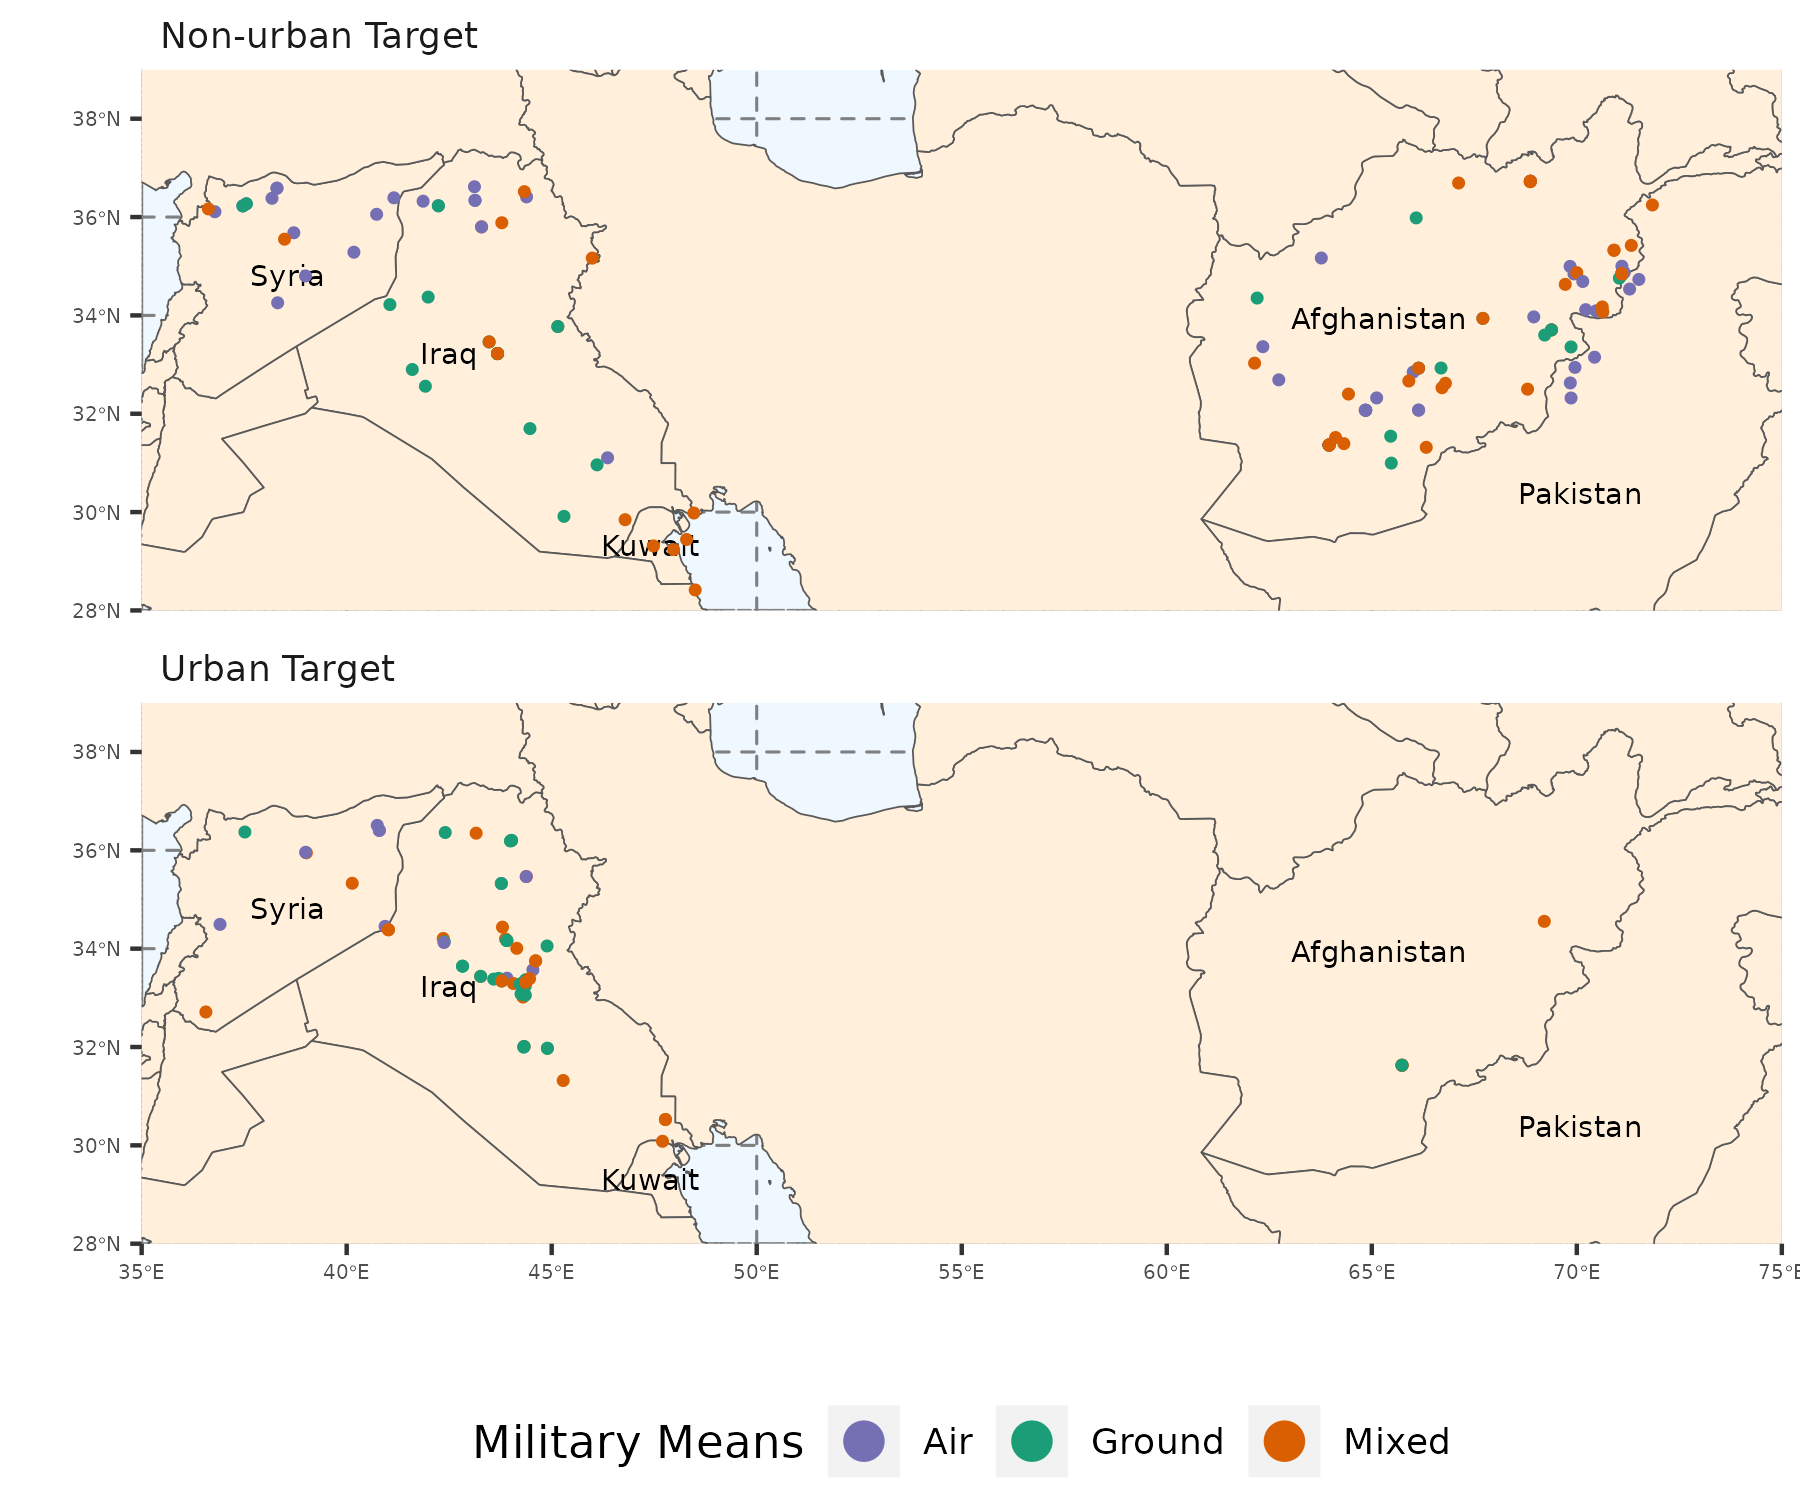
\includegraphics[width = \textwidth]{fig-map-1.png}}
		\label{fig:fig-map-1}
		\vspace{0.1 in}
	\end{center}
\end{figure}
\setstretch{2.0}

\clearpage
\setstretch{1.0}
\newpage
\begin{figure}[h]
	\begin{center}
		\caption{Social Network Plots of Select Conflicts}
		{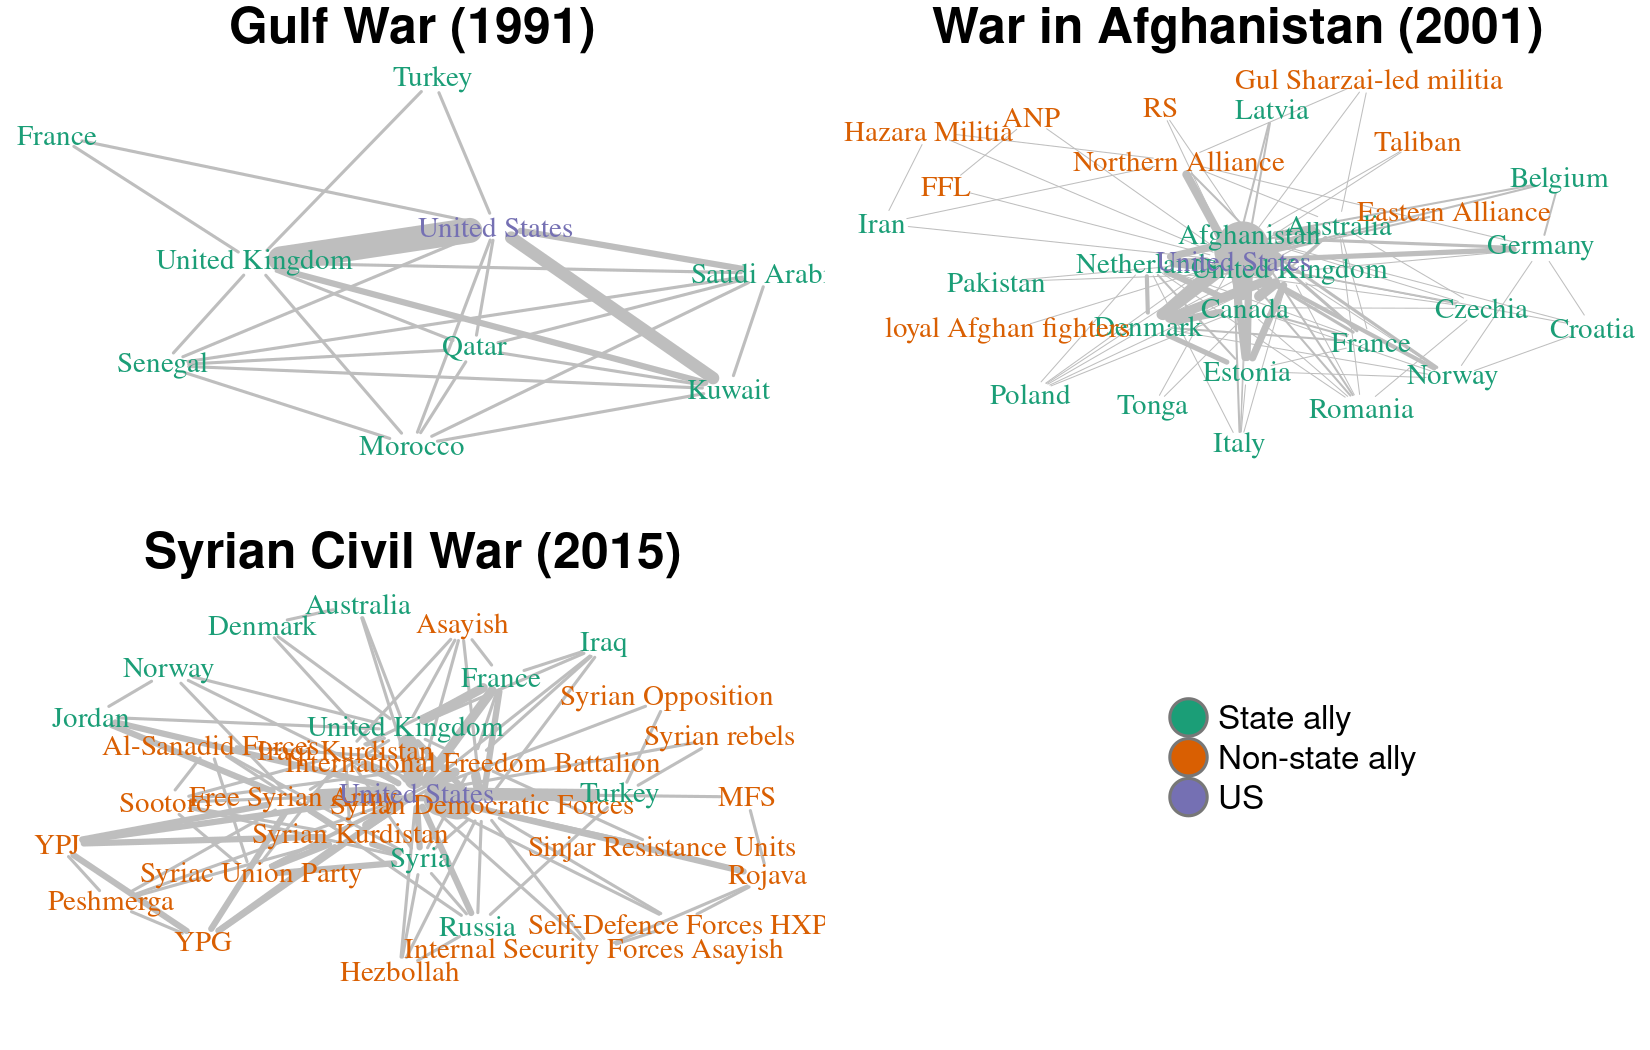
\includegraphics[width = \textwidth]{fig-actors-1.png}}
		\label{fig:fig-actors-1}
		\vspace{0.1 in}
	\end{center}
\end{figure}
\setstretch{2.0}

\clearpage

\newpage

\bibliography{MONSTr.bib}

\end{document}